\documentclass[12pt]{article}
\setlength{\oddsidemargin}{0in}
\setlength{\evensidemargin}{0in}
\setlength{\textwidth}{6.5in}
\setlength{\parindent}{0in}
\setlength{\parskip}{\baselineskip}

\usepackage{xcolor}
\usepackage{amsmath,amsfonts,amssymb}
\usepackage{qtree}
\usepackage{enumerate}
\usepackage{multirow}
\usepackage{graphicx}
\usepackage{forest}
\usepackage{colortbl}

\begin{document}

CSCI 4448 Spring 2016 \hfill Project Write-up 2\\

\hrulefill
%%%%%%%%%%%%%%%%%%%%%%%%% SECTION 1  %%%%%%%%%%%%%%%%%%%%%%%%%
\begin{center}
  \textbf{Business Requirements} \\
\begin{tabular}{ l  l  l  l  l  }
  \textbf{ID}  & \textbf{Requirement} & \textbf{Topic Area} & \textbf{Actor} & \textbf{Priority} \\  \rowcolor[gray]{.95} \hline
  BR-001 & Ingredients must be able to include sponsor links & Advertising & All & Medium \\  
  BR-002 & Collect user data for later processing & Reporting & Admin & Medium \\  \rowcolor[gray]{.95}
  BR-003 & Replication factor of 3 for data consistency & Database & Admin & High \\ 

\end{tabular}
\\
  \vspace{1cm}


 \textbf{User Requirements} \\
\begin{tabular}{ l  l  l  l  l  }
  \textbf{ID}  & \textbf{Requirement} & \textbf{Topic Area} & \textbf{Actor} & \textbf{Priority} \\  \rowcolor[gray]{.95}  \hline
  UR-001 & User can search ingredients by category & Interface & User & High \\  
  UR-002 & User can search ingredients by query & Interface & User & High \\  \rowcolor[gray]{.95}
  UR-003 & User can enter dietary restrictions & Interface & User & Medium \\  
  UR-004 & User can enter an optimal price range & Interface & User & Medium \\  \rowcolor[gray]{.95}
   UR-005 & User can save a dietary preference/restriction & User & Medium \\ 
  UR-006 & User can select importance value of dietary restriction & Interface & User & Medium \\ \rowcolor[gray]{.95}
  UR-007 & User can generate recipe list at any point & Interface & User & Medium \\
  UR-008 & User can remove an ingredient from their list & Functionality & User & Medium \\
\end{tabular}
\\
  \vspace{1cm}
  \textbf{Non-Functional Requirements}
\begin{tabular}{ l  l  l  l  l  }
  \hline
  \textbf{ID}  & \textbf{Requirement} & \textbf{Topic Area} & \textbf{Actor} & \textbf{Priority} \\  \rowcolor[gray]{.95}
  NFR-001 & Show 10 recipes upon search  &  Interface & User & Low  \\  
  NFR-002 & Return at least 3 hits in under one second & Media & User &  Medium\\  \rowcolor[gray]{.95}
  NFR-003 & Less than one second load time for inital website &  Website & All & High \\ 
  NFR-004 & Recent database results cached locally & Database & User & Low \\  \rowcolor[gray]{.95}
  NFR-005 & Set partition size for Database & Database & Admin & Low \\ 
\end{tabular}
\end{center}

\newpage
\textit{Database: } We will be using Cassandra DB so that we can easily delegate multi-factor replication and partition management. We will be hosting our database using
Amazon S3 which easily integrates a Cassandra deployment. \\
\vspace{1cm} \\
\textit{Data Persistance: } We will have a static list of recipe names with ingredients lists which will persist. We will query the database and MapReduce based on the ingredients
provided by the user to provide a list of the 10 best matches. We will have a separate partition of data persistance allocated for user ingredients data. 

\newpage
\begin{figure}
  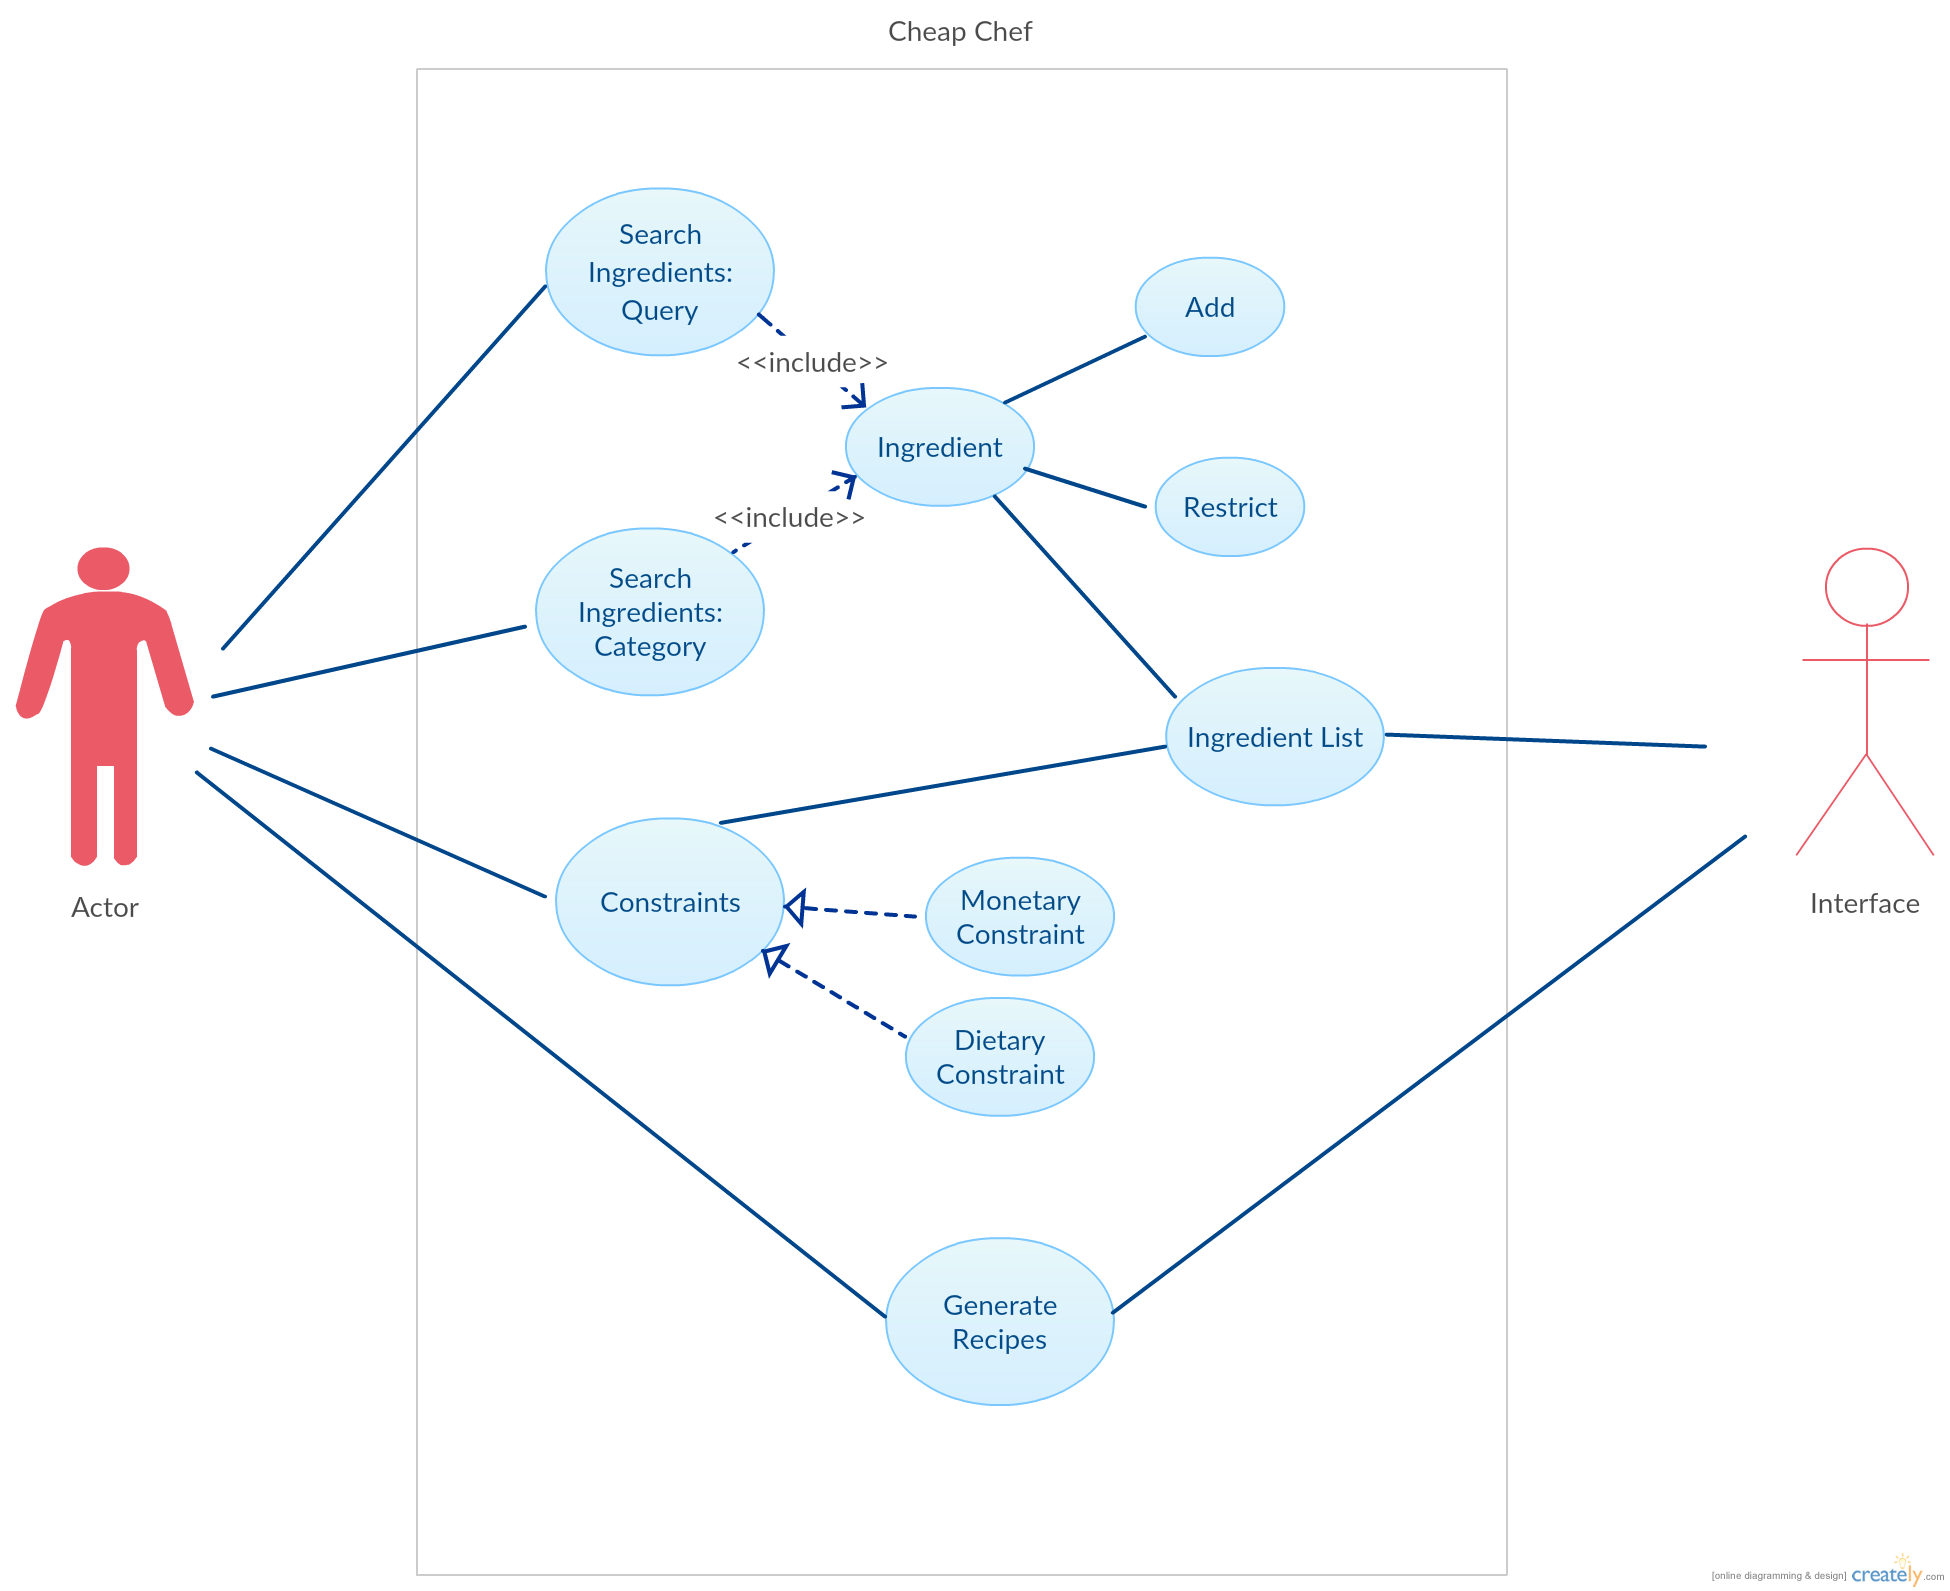
\includegraphics[width=\linewidth]{usecases.png}
  \caption{Use Cases}
  \label{fig: usecases}
\end{figure}

\newpage
\begin{center}
  \textbf{Class Diagram}
\end{center}

\end{document}
